\documentclass{beamer}
\usepackage{./presentation_style}
\mode<presentation>{
    \usetheme{Madrid}
%    \usetheme{Pittsburgh}
%    \usetheme{metropolis}
}





% To remove the footer line in all slides 
\setbeamertemplate{footline}

% To replace the footer line in all slides with a simple slide count 
\setbeamertemplate{footline}[page number]

% To remove the navigation symbols from the bottom of all slides 
\setbeamertemplate{navigation symbols}{} 


%\setbeamersize{text margin left=5mm,text margin right=5mm} 
%\addtobeamertemplate{frametitle}{}{\vspace{-3em}} % decrease




% ---------- Title Page ----------------
 % The short title appears at the bottom of every slide, the full title is only on the title page
\title{Microlocal Analysis \\ 
    \large with Applications to Non-Elliptic Fredholm Problems}

\author{Edmund Lau \\
Supervised by: Dr Jesse Gell-Redman} 

% Your institution as it will appear on the bottom of every slide, may be shorthand to save space
\institute[Unimelb] {
    The University of Melbourne \\ % institution for the title page
    \medskip
    \textit{elau1@student.unimelb.edu.au} % email address
}

\date{19 October 2018} 

\begin{document}
    
% ------------------------------------------ Title Frame 
\begin{frame}
\titlepage 
\end{frame}






%######################################### Section: Introduction
\section{Introduction} 
%------------------------- Frame : Introduction 1
\begin{frame}{Introduction}
A linear partial differential operator in $\R^n$ : 
\begin{equation}
P = P(x, D_x) = \sum_{\abs{\alpha} \leq k} c_\alpha(x) D^\alpha_x 
\end{equation}
\pause
where 
\begin{align*}
\alpha &= (\alpha_1, \alpha_2, \dots, \alpha_n) \in \N^n \tag*{ multi-index } \\
\abs{\alpha} &= \alpha_1 + \alpha_2 + \dots + \alpha_n \tag*{order of multi-index} \\
c_\alpha &\in C^\infty_\infty(\R^n) \tag*{ bounded  smooth functions} \\
D_{x_i} &= -i \p_{x_i} \\
D_x^\alpha & = \brac{-i \p_{x_1}}^{\alpha_1}\brac{-i \p_{x_2}}^{\alpha_2} \dots \brac{-i \p_{x_n}}^{\alpha_n} 
\end{align*}
\end{frame} 
% ------------------------- End Frame 


%------------------------- Frame : Introduction 2
\begin{frame}{Introduction}
A linear partial differential equation (PDE) : 

\begin{equation}
P u = f
\end{equation}

\onslide<1->
Smooth solution and forcing: 
\begin{align*}
C^\infty(\R^n) \ni u, \, f : \R^n \to \C 
\end{align*}

\onslide<2-> 
Weak solution and forcing: 
\begin{align*}
\sch'(\R^n) \ni u, \, f : \sch(\R^n) \to \C 
\end{align*}
\begin{align*}
u \in \sch(\R^n)  \iff 
 u \in C^\infty \text{ and }  \sup_{x} \abs{x^\beta D^\alpha_x u(x)} < \infty 
\end{align*}


\onslide<3->
Example: 
\begin{align*}
&\Delta u = - \p_{x_1}^2 u - \dots - \p_{x_n}^2 u  = \delta \tag*{Laplace operator} \\
&\Box u = \p_{t}^2 u - \p_{x_1}^2 u - \dots - \p_{x_n}^2 u  = 0 \tag*{Wave operator} 
\end{align*}

\end{frame} 
% ------------------------- End Frame 


%------------------------- Frame : Introduction 3
\begin{frame}{Introduction}
%Given a PDE, $P u = f$, the all important questions are 
\begin{description}
    \item[Existence]<1-> Can we find a solution $u$? 
    \item[Uniqueness ]<2->  If that's possible,  is it the only one? 
    \item[Regularity ]<3-> Is $u$ continuous? differentiable? smooth? rapid decreasing? \\
\end{description}

\onslide<4> We will use the \textbf{Fredholm} theory  to tackle all three simultaneously! 

\end{frame} 
% ------------------------- End Frame 



% ------------------------------------------ Content Overview 
\begin{frame}{Overview}
\tableofcontents
\end{frame}

%######################################### Section: Fredholm operators
\section{Fredholm Operators and Regularity} 


%------------------------- Frame : Fredholm 1 
\begin{frame}{Fredholm Operators}
\begin{definition}[Fredholm operators]
    A continuous linear operator $T : \X \to\Y$ between Banach spaces $\X$ and $\Y$ is Fredholm, if 
    \begin{itemize}
        \item $T$ has closed range, i.e. $T(\X)$ is closed in $\Y$, 
        \item $\ker(T) \subset \X $ is finite dimensional, 
        \item $\coker(T) := \Y / T(\X)$ is finite dimensional. 
    \end{itemize}
\end{definition}
\pause
Suppose $Tx = y$ for a given $y \in \Y$. 
\begin{description}
    \item[Existence] a solution $x \in \X$ exist if and only if  $y \not \in \coker(T)$. 
    \item[Uniqueness] the solution is unique if and only if $\ker(T) = 0$. 
\end{description}
\pause
$T$ Fredholm \\
$\implies$ existence and uniqueness is a finite dimensional linear algebraic problem. 

\end{frame}

%------------------------- Frame : Fredholm estimates
\begin{frame}{Fredholm Estimate}
In PDE, we would like  topological / algebraic statements $\leadsto$ estimates. 
\pause
\begin{theorem} \label{theorem: fredholm estimates}
    Let $\X$, $\Y$, $\mathcal{Z}$ be Banach spaces.  If 
    \begin{itemize}
        \item $T : \X \to \Y$ is continuous, 
        \item $\X$ is compactly contained in $\mathcal{Z}$, i.e.  $\iota : \X\hookrightarrow \mathcal{Z}$ is compact, 
        \item for all $u \in \X$, there exist $C > 0$ such that the  following estimate hold
        \begin{align}
        \norm[x]_\X \leq C \brac{\norm[Tx]_\Y + \norm[u]_\mathcal{Z}}
        \end{align}
    \end{itemize}
    then 
    \begin{itemize}
        \item the image, $T(\X)$ is closed, and
        \item $T$ has finite dimensional kernel. 
    \end{itemize} 
\end{theorem}


\end{frame} 
% ------------------------- End Frame 

%------------------------- Frame : Fredholm problem 
\begin{frame}{Constructing a \textit{Fredholm problem}} 
What's a Fredholm differential operator? $\dots $ what's $\X$ and $\Y$? 
\begin{block}{Fredholm Problem}
    Given a differential operator $P$, can we construct solution spaces $\X$ and $ \Y$,  so that $$P : \X \to \Y$$ is Fredholm? 
\end{block}
\pause 

What's the link to \textit{regularity}? Answer: Sobolev spaces. 

\end{frame} 
% ------------------------- End Frame 

%------------------------- Frame : Sobolev space
\begin{frame}{Sobolev Space}
\begin{definition}
    The Sobolev space of order $k \in \N$ on $\R^n$,  $H^k(\R^n) \subset \sch'(\R^n)$  is defined by 
    \begin{align*}
    u \in H^k(\R^n) 
    &\iff D^\alpha u \in L^2(\R^n) \text{ whenever } \abs{\alpha} \leq k\\
    &\iff \sym[\xi]^k \widehat{u}(\xi) \in L^2(\R^n). 
    \end{align*}
\end{definition}

\begin{align*}
\sym[\xi] &:= \brac{1 + \abs{\xi}^2}^{1/2} = \brac{1 + \abs{\xi_1}^2+ \dots + \abs{\xi_n}^2}^{1/2} \\
\widehat{u}(\xi) &:= \F u(\xi)  = \frac{1}{(2\pi)^{n/2}} \int e^{-ix \cdot \xi} u(x)\d[x] 
\end{align*}

Hilbert space structure that keeps track of (global) regularity data of $u$. 
\begin{align*}
    \norm[u]_{H^k} = \underbrace{\norm[u]_{L^2}}_{\text{ global decay}}  + \underbrace{\sum_{\abs{\alpha} \leq k} \norm[D^\alpha u ]_{L^2} }_{\text{ $k$ times differentiable}} 
\end{align*}

\end{frame} 


%------------------------- Frame : Sobolev space generalisation 
\begin{frame}{Sobolev Space on Compact Manifold}
Let $M$ be a smooth compact $n$-manifold without boundary (i.e. closed manifold), $s \in \R$, $u \in \brac{C^\infty(M)}'$, then 
\begin{align*}
u \in H^s(M) \iff \brac{\chi \cdot  u} \circ \Phi^{-1} \in H^s(U)
\end{align*} 
for any chart $\Phi : \widetilde{U} \to U \subset \R^n$ and smooth bump function $\chi \in C^\infty(M)$ compactly supported in the chart domain $\widetilde{U}$. \\[3em]
\pause 
Henceforth, $M$ is either $\R^n$ or a closed $n$-manifold. 
\end{frame} 
% ------------------------- End Frame 

%------------------------- Frame : General strategy
\begin{frame}{General Strategy}
%Given differential operator $P$ on manifold $M$: 
\begin{block}{Reduced question} 
    Existence, uniqueness, regularity $ \leadsto $ can we find $\X \subset H^s(M)$, $\Y \subset H^{s'}(M)$ so that 
    \begin{align*}
    P: \X \to \Y 
    \end{align*}
    is Fredholm? 
\end{block}
On closed manifold, $H^s(M) \Subset H^{s - \epsilon}(M)$ for any $\epsilon > 0$. 
\begin{block}{General Strategy}
    Prove that for \textbf{any} $s, N \in \R$, there exist $C > 0$, 
    \begin{align*}
    \norm[u]_{H^s} \leq C \brac{\norm[Pu]_{H^{s'}} + \norm[u]_{H^{N}}}. 
    \end{align*}    
\end{block}

\end{frame} 
% ------------------------- End Frame 


%######################################### Section: Elliptic case
\section{``Elliptic operators are Fredholm"} 
%------------------------- Frame : Elliptic regularity
\begin{frame}{``Elliptic operators are Fredholm"} 
How do we get such an estimate? 

% ------------------------- End Frame 
\begin{theorem}[Elliptic regularity]
    Let $P$ be an order $m \in \R$ \textcolor<2->{red}{\only<2->{\LARGE} elliptic} \only<2->{\textcolor<2->{red}{\Large (pseudo-)}} differential operator on an $n$-manifold, $M$. Suppose we know \textit{a priori} that $u \in H^{N}(M)$ for some $N \in \R$. Then, for any $s \in \R$
    \begin{align*}
    (f = ) Pu \in H^{s}(\R^n) \implies u \in H^{s + m}(\R^n)
    \end{align*}
    and $u$ satisfies the estimates: $\exists C > 0$
    \begin{align*}
    \norm[u]_{H^{s + m}} \leq C \brac{\norm[Pu]_{H^s} + \norm[u]_{H^N}}. 
    \end{align*}
\end{theorem}

\end{frame} 


%------------------------- Frame : Elliptic operator
\begin{frame}{Elliptic operator}
Elliptic operators generalise the Laplace operator: $\Delta \uncover<2->{+1}$. \\
\onslide<3-> 
Fourier transform + integration by parts $\implies$ 
\begin{align*}
\brac{\Delta + 1} u(x) = \frac{1}{(2\pi)^n} \int e^{i(x - y) \cdot \xi} \brac{1 + \abs{\xi}^2} u(y) \d[y]  \d[\xi]
\end{align*}
\onslide<4-> 
We expect the existenc of an inverse $\dots$ 
\begin{align*}
&\brac{\Delta + 1}^{-1} \brac{\Delta + 1} u(x) \\
&= \frac{1}{(2\pi)^n} \int e^{i(x - y) \cdot \xi} \underbrace{\brac{1 + \abs{\xi}^2}^{-1} \brac{1 + \abs{\xi}^2}}_{= 1} u(y) \d[y]  \d[\xi] = u(x) 
\end{align*}
$\brac{1 + \abs{\xi}^2}^{\pm 1} $ are the \textbf{symbols} for $\brac{\Delta + 1}^{\pm 1} $. 
\end{frame} 

%------------------------- Frame : Pseudodifferential operator
\begin{frame}{Pseudodifferential operator}
Question: What is $\brac{\Delta + 1}^{-1}$? Answer: \textbf{pseudo}differential operator. 
\begin{align}
P(x, D_x) u = \frac{1}{(2\pi)^n} \int e^{i(x - y) \cdot \xi} p(x, \xi) u(y) \d[y] \d[\xi]  \label{eq: action of symbol} 
\end{align}
\onslide<2-> 
\begin{definition} A smooth function $p(x, \xi) \in C^\infty(\R^{n}; \R^n)$ is a symbol of order $m \in \R$, i.e. $p \in S^{m}_\infty(\R^{n}; \R^n)$, if
    \begin{align*}
    \abs{D^{\alpha}_x D^\beta_\xi p(x, \xi)} \leq C_{\alpha, \beta, \gamma}  \sym[\xi]^{m - \abs{\beta}}, \quad C_{\alpha, \beta}  > 0
    \end{align*}
    for any multi-index $\alpha, \beta \in \N^n$. \\
    
    A pseudodifferential operator, $P \in \Psi^{m}_{\infty}(\R^n)$ of order $m$ with (left reduced) symbol $p \in S^{m}_\infty(\R^{n}; \R^n)$ has action on $u \in \sch'(\R^n)$ given by (\ref{eq: action of symbol}). 
\end{definition}
\end{frame} 

%------------------------- Frame : Prove of elliptic regularity
\begin{frame}{Proof sketch of elliptic regularity}
\begin{theorem}
    The total spaces $\cup_{m} S^{m}_\infty(\R^{n}; \R^n)$ and $\cup_{m} \Psi^{m}_{\infty}(\R^n)$ form filtered *-algebra over $\C$. If $P \in \Psi^{m}_{\infty}(\R^n)$ for some $m \in \R$, 
    \begin{enumerate}
        \item $P : H^{s}(\R^n) \to H^{s - m}(\R^n)$ is continuous for any $s \in \R$. 
        \item If $P$ is \textbf{elliptic} of order $m$, i.e. its symbol $p$ satisfies
        \begin{align*}
        \abs{p(x, \xi)} \geq \epsilon \sym[\xi]^m \tag*{ in $\abs{\xi} > \epsilon$ for some $\epsilon > 0$ } 
        \end{align*}
        then there exist \textit{parametrix} $Q \in \Psi^{-m}_{\infty}(\R^n)$ such that $QP - 1: H^{s} \to H^{s'}$ is continuous for any $s, s' \in \R$. 
    \end{enumerate}
\end{theorem}
\onslide<2->
\textit{Proof sketch (elliptic regularity). } 
\only<2>{$$u = QP u -  \brac{QP - 1} u$$} 
\onslide<3->
\begin{align*}
\norm[u]_{H^{s + m}} 
&\leq \underbrace{\norm[QPu]_{H^{s + m}}}_{\leq C \norm[Pu]_{H^s}} + \underbrace{\norm[\brac{QP - 1}u]_{H^{s +m}}}_{\leq C \norm[u]_{H^N}}
\end{align*}
using continuity $Q: H^{s +m} \to H^{s}$ and $(QP - 1): H^{s + m} \to H^{N}$.  

\end{frame} 



%######################################### Section: Non-elliptic case
\section{A Non-elliptic Fredholm problem}

%------------------------- Frame : Non-Elliptic Fredholm Problem
\begin{frame}{Non-elliptic Fredholm problem}
Recent work by \cite{Vasy, Gell-Redman} show that we can construct Fredholm problem for \textbf{non-elliptic} operators too! \\
We'll illustrate by sketching the proof for a pertubation of the  wave operator 
\begin{align*}
\Box := \p_t^2 - \sum_{j = 1}^{n -1} \p_{x_j}^2
\end{align*}
on the $1 + n$-torus, 
\begin{align*}
\T^{1 + n} := \S^1_t \times  \underbrace{\S^1_{x_1} \times \S^1_{x_2} \times \dots \times \S^1_{x_n}}_{n} 
\end{align*}
where $\S^1 := [0, 1] / (0 \sim 1)$ is the circle and $(t, x) = (t, x_1, \dots, x_n)$ are the local coordinates on $\T^{1 + n}$. 
\end{frame} 
% ------------------------- End Frame 

%------------------------- Frame : Main theorem
\begin{frame}{Main theorem}
\begin{theorem}
    There exist a perturbation $Q$ of the wave operator $\Box$ on $\T^{1 + n}$ and a subspace $\X^s \subset H^{s}(\T^{1 +n})$ for each $s \in \R$, such that the operator: 
    \begin{align*}
    (\Box - iQ): \mathcal{X}^s \to H^{s - 1}(\T^n)
    \end{align*}
    is Fredholm. 
\end{theorem}

\end{frame} 
% ------------------------- End Frame 

%------------------------- Frame : Ingredients
\begin{frame}{Two Major Ingredients}
\begin{theorem}[Microlocal elliptic regularity]
        Let $A \in \Psi^{m}_{\infty}(\R^n)$ and $u \in \sch'(\R^n)$. If for some $Q' \in \Psi^{0}_{\infty}(\R^n)$, $Q'Au \in H^{s}(\R^n)$, then for any other $Q \in \Psi^{0}_{\infty}(\R^n)$ such that $\WF'(Q) \subset \Ell^m(A) \cap \Ell^0(Q')$ we have $Qu \in H^{s + m}(\R^n)$ and it satisfies the estimate: $\forall N \in \R$, $\exists C > 0$ 
        \begin{align*}
        \norm[Qu]_{H^{s +m}} \leq C \brac{\norm[Q'Au]_{H^s} + \norm[u]_{H^N}}. 
        \end{align*}
\end{theorem}
\begin{theorem}[Propagation of singularities] \label{theorem: propagation of singularity estimates}
    Let $P \in \Psi^{m}_{\infty}(\R^n)$ is a properly supported pseudodifferential operator with polyhomogeneous principal $\sigma_m(P) = p - iq$ with real $p, q$. If we have $A, B, B' \in \Psi^{0}_{\infty}(\R^n)$ and $q \geq 0$ on $\WF'(B')$ and every $(x, \xi) \in WF'(A)$ is in the integral curve of $H_p$ originating from $\Ell^0(B)$, then for all $s, N \in \R$ and $u \in C^\infty(\R^n)$, there exist $C > 0$ such that 
    \begin{align*}
    \norm[Au]_{H^s} \leq C\brac{\norm[Bu]_{H^s} + \norm[B'Pu]_{H^{s - m + 1}} + \norm[u]_{H^{-N}}}. 
    \end{align*}
\end{theorem}
\end{frame} 
% ------------------------- End Frame 


%------------------------- Frame : 
\begin{frame}{Constructions}
First, we define a bump functions in the time dimension $\chi(t)$ as below: 

\begin{center}
    \begin{tikzpicture}[scale=0.8]
    \draw [] (0, 0) rectangle (8, 8);
    \node at (8.3, -0.1) {$x$};
    \node at (-0.1, 8.3) {$t$}; 
    \pause 
    
    \draw[pattern=north west lines, pattern color=blue, opacity=0.5] (0, 0) rectangle (8, 2.5);
    \draw[pattern=north west lines, pattern color=blue, opacity=0.5] (0, 5.5) rectangle (8, 8);
    \node at (8.7, 2.5) {$\delta + \delta'$}; 
    \node at (9.1, 5.5) {$1 - \delta - \delta'$};
    \node [fill=white]  at (4, 7) {$U_1 :=  \set{\chi(t) \equiv 1}$ };
    \node [fill=white] at (4, 1) {$U_1$};
    
    \pause 
    
    \draw [->, thick] (-0.5, 0) -- (-3, 0); 
    \draw [->, thick] (-0.5, 0) -- (-0.5, 8);
    \draw [-, thick] (-2.5, 0.1) -- (-2.5, -0.1);
    \node at (-3.3, -0.3) {$\chi(t)$};
    \node at (-2.5, -0.3) {1}; 
    
    \draw (-2.5, 0) -- (-2.5, 2);
    \draw[rounded corners=8pt] (-2.5, 2) -- (-2.5, 2.24) -- (-1, 2.25) -- (-0.5, 2.5);
    \node at (-2.5, 8) (right start) {};
    
    \draw (-2.5, 8) -- (-2.5, 8 - 2);
    \draw[rounded corners=8pt] (-2.5, 8 - 2) -- (-2.5, 8 - 2.24) -- (-1, 8 - 2.25) -- (-0.5, 8 - 2.5);
    
    \draw  [dashed] (-2.5, 2) -- (8.1, 2);
    \draw  [dashed] (-2.5, 6) -- (8.1, 6);
    \draw  (-0.5, 5.5) -- (8.1, 5.5);
    \draw  (-0.5, 2.5) -- (8.1, 2.5);
    
    
    \node at (8.6, 6) {$1 - \delta$};
    \node at (8.6, 2) {$\delta$};
    \pause 
%    
%    
%    \draw[pattern=north east lines, pattern color=red, opacity=0.5] (0, 2.25) rectangle (8, 5.75); 
%    \draw [thick] (0, 2.25) -- (8, 2.25); 
%    \draw [thick] (0, 5.75) -- (8, 5.75); 
%    \node at (-0.2, -0.2) {$0$};
%    \node [fill=white] at (4, 4) {$U_2 = $ a neighbourhood of $\set{\chi(t) = 0}$};
    \end{tikzpicture}
\end{center}
\end{frame} 
% ------------------------- End Frame 

%------------------------- Frame : 
\begin{frame}{Constructions}
Define in local coordinates
\begin{align*}
Q = \chi(t) \p_t^2 \implies \Box - iQ = \brac{1 - i\chi(t)} \p_{t} - \sum_{i = 1}^n \p_{x_i}^2 
\end{align*}
with principal symbol 
\begin{align*}
p & := \sigma_2(\Box) = \tau^2 - \abs{\xi}^2 \\
q & := \sigma_2(Q) = \chi(t) \tau^2 \implies \sigma_2(\Box - iQ) = \brac{1 - i\chi(t)} \tau - \abs{\xi}^2. 
\end{align*}

%\begin{center}
%    \begin{tikzpicture}[scale=0.3]
%    \draw[->] (0, 0) -- (6, 0);
%    \node at (5.9, -0.5) {$x$}; 
%    \draw[->, thick] (0, 0) -- (0, 6);
%    \node at (-0.2, 6.2) {$t$};  
%    
%    \node at (3, 2.6 ) {$(t_0, x_0)$}; 
%    \draw (3, 2.9) -- (3, 3.1); 
%    
%    
%    \draw [->] (1, 1) -- (5, 5); 
%    \draw [<-] (1, 5) -- (5, 1); 
%%    \node at (5.5, 5.5) {$\set{x - t = x_0}$}; 
%%    \node at (1.5, 5.5) {$\set{x + t = x_0}$}; 
%    \end{tikzpicture}
%\end{center}

\end{frame} 
% ------------------------- End Frame 

%------------------------- Frame : 
\begin{frame}{Hamilton flow of $\sigma_2(\Box)$ }
Hamiltonian flow:
\begin{align*}
\exp(sH_ p)(t, x, \tau, \xi) = (t + s\tau, x + s \xi, \tau, \xi)
\end{align*}
\begin{center}
    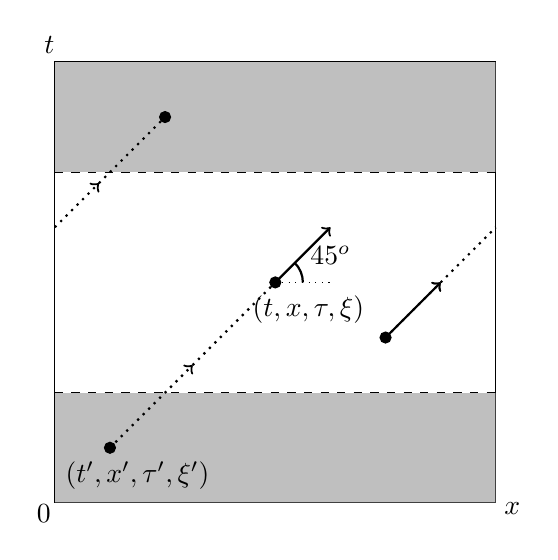
\begin{tikzpicture}[scale=0.7]
    \draw [] (0, 0) rectangle (8, 8);
    \fill [gray, opacity=0.5] (0, 0) rectangle (8, 2);
    \fill [gray, opacity=0.5] (0, 6) rectangle (8, 8);
    \draw [dashed] (0, 2) -- (8, 2);
    \draw [dashed] (0, 6) -- (8, 6);
    
    \draw [fill=black] (4, 4) circle [radius = 0.1]; 
    \draw [->, thick] (4, 4) -- (5, 5);
    \node at (4.6, 3.5) {$(t, x, \tau, \xi)$}; 
    
    
    \draw [fill=black] (1, 1) circle [radius = 0.1]; 
    \draw [->, thick, dotted] (1, 1) -- (2.5, 2.5);
    \draw [thick, dotted] (2.5, 2.5) --  (4, 4); 
    \node at (1.5, 0.5) {$(t', x', \tau', \xi')$}; 
    
    
    \draw [dotted] (4, 4) -- (5, 4);
    \draw [thick] (4.5, 4) arc (0:45:0.5); 
    \node at (5, 4.5) {$45^o$}; 
    
    \node at (8.3, -0.1) {$x$};
    \node at (-0.1, 8.3) {$t$}; 
    \node at (-0.2, -0.2) {$0$};
    
    
    
    \draw [fill=black] (6, 3) circle [radius = 0.1]; 
    \draw [->, thick] (6, 3) -- (7, 4);
    \draw [->, thick, dotted] (6, 3) -- (7, 4);
    \draw [thick, dotted] (7, 4) -- (8, 5);
    \draw [->, thick, dotted] (0, 5) -- (0.8, 5.8); 
    \draw [thick, dotted] (0.8, 5.8) -- (2, 7); 
    \draw [fill=black] (2, 7) circle [radius = 0.1];
    \end{tikzpicture}
\end{center}
\end{frame} 

% ------------------------- End Frame 


% ------------------------------------------ Sandbox frame
\appendix
\section*{sandbox}

Fourier analysis relates the (global) regularity of functions to their fourier transform. e.g. in the 'superposition of wave' picture, only waves with high frequency can approximate jump discontinuity, linking continuity with the decay of fourier coefficients. 
Microlocal analysis also keeps track of the direction of decay. 
\begin{theorem}[Rank-nullity]
    If $T : V \to W$ be a linear operator between finite dimensional vector space $V$ and $W$, then 
    \begin{align*}
    \mathrm{Ind}(T) := \dim \ker T - \dim \coker T = \dim W - \dim V. 
    \end{align*}
\end{theorem}
\begin{theorem}[Atiyah-Singer index theorem]
    Given
    \begin{itemize}
        \item $X$ a smooth comapct manifold, 
        \item $E, F$ smooth vector bundles over $X$, 
        \item $P : \Gamma(E) \to \Gamma(F)$ be an elliptic differential operators between the space of sections of $E$ and $F$. 
    \end{itemize}
    Then, $P$ is Fredholm and its Fredholm index is related to its topological index. 
\end{theorem}


\end{document}


%\begin{frame}{Fredholm operators}
%\begin{align*}
%T x = y \quad x \in X, \, y \in Y
%\end{align*}
%\begin{itemize}
%    \item $\dim \coker(T) < \infty $ means that solutions exist if and only if 
%    $$\omega_1(y) = \omega_2(y) = \dots \omega_n(y) = 0$$ 
%    where $\set{\omega_i}_{i = 1}^n$ is any basis of $\coker(T)$. \todo{with isomorphism to the perpendicular space}
%    
%    \item $\dim \ker(T) < \infty$ means that solution is unique up to addition of element in a finite dimensional space. 
%    
%    \item $T$ is invertible modulo compact operators (limits of finite rank operators). 
%\end{itemize}
%
%\end{frame}


%\begin{frame}{Fredholm Index}
%\begin{definition}
%    The index of a Fredholm operator $T$ is defined by
%    \begin{align*}
%    \ind(T) := \dim \ker(T) - \dim \coker(T). 
%    \end{align*}
%\end{definition}
%\begin{itemize}
%    \item $\ind : \mathrm{Fred}(X, Y) \to \Z$ is a continuous map. 
%    \item Unlike kernel and cokernel themselves, $\ind$ is well-behaved. \todo{example on the circle.}
%    \item \todo{something about Atiyah-Singer index which only works for elliptic diff on compact manifolds} 
%\end{itemize}
%
%
%\end{frame}
%
%
%
%\begin{frame}{Fredholm differential operators}
%\begin{theorem} \label{theorem: fredholm estimates}
%    Let $V$, $W$, $Y$ be Banach spaces, $T \in \L(V, W)$ and $K \in \K(V, Y)$. If for all $u \in V$, the estimate 
%    \begin{align*}
%    \norm[u]_V \leq C \brac{\norm[Tu]_W + \norm[Ku]_Y}
%    \end{align*}
%    holds for some positive real constant $C \in \R_{> 0}$, then the image, $T(V)$ is closed, and $T$ has finite dimensional kernel. 
%\end{theorem}
%
%Suppose we can show that the differential operator $P$ is Fredholm as a map 
%\begin{align*}
%P : H^{s} \to H^{s - m}
%\end{align*}
%
%\begin{align*}
%Pu = f \quad f \in H^s(M), u \in \sch'
%\end{align*}


% ------------------------- End Frame 

% ------------------------- End Frame 
% ------------------------- End Frame 
%\begin{frame}{``Ellitptic Operators are Fredholm"}
%\begin{example}[Laplacian]
%    $\Delta: H^{s} \to H^{s - 2}$
%    \begin{align*}
%    \norm[u]_{H^{s + 2}} \leq C \brac{\norm[\Delta u]_{H^s} + \norm[u]_{L^2}}. 
%    \end{align*}
%\end{example}
%
%\begin{proposition}
%    Let $A \in \Psi^{m}_{\infty}(\R^n)$ be elliptic and $u \in H^{N}(\R^n)$ for some $N \in \R$. Then, for any $s \in \R$
%    \begin{align*}
%    Au \in H^{s}(\R^n) \implies u \in H^{s + m}(\R^n)
%    \end{align*}
%    and $u$ satisfies the estimates: $\exists C > 0$
%    \begin{align*}
%    \norm[u]_{H^{s + m}} \leq C \brac{\norm[Au]_{H^s} + \norm[u]_{H^N}}. 
%    \end{align*}
%\end{proposition}
%
%
%\todo{
%    Elliptic regularity estimate. (compact and non-compact manifold case). 
%}
%
%\end{frame}
